%!TeX root = main.tex
\chapter{DIE Klasse der Fourier-Transformationen}
In diesem Kapitel werden Beispiele einer speziellen Klasse von $\cD$-Moduln
diskutiert. Dazu wird im folgendem zu einem Beispiel unter anderem explizit der
Beweis aus \cite{sabbah_cimpa90} zur Levelt-Turrittin-Zerlegung nachvollzogen.

Es wird zunächst ein allgemeines Rezept gegeben, welches zu gegebenem $\phi$
D-Moduln ergibt. Im laufe des Kapitels werden immer speziellere $\phi$
betrachtet und zuletzt wird für konkrete Beispiele eine explizite Rechnung
gegeben.

\section{Rezept für allgemeine $\phi$} \label{sec:allgemeinProblem}
Hier wollen wir nun eine Spezielle Klasse von Meromorphen Zusammenhängen, die
die durch das folgende Rezept entstehen.
\begin{enumerate}
\item Wähle zunächst ein $\phi$
$\in\{\phi=\sum_{k\in I}\frac{a_k}{t^{k}}|I\subset\N\mbox{ endlich}
,a_k\in \C\}$
aus
\item und beginne mit $\sE^{\phi}$. Es gilt
\begin{align*}
\sE^{\phi} &= \cD_{\hat L}/\cD_{\hat L}\cdot (\partial_t-\frac{d}{dt}\phi(t))
\\&=\cD_{\hat L}/\cD_{\hat L}\cdot (\underset{\in\C[t]\subset\cD_{\hat L}^*}
    {\underbrace{\mbox{\textbf{Hauptnenner von $\frac{d}{dt}\phi(t)$ }}}}
  \cdot (\partial_t-\frac{d}{dt}\phi(t)))
\\&=\cD_{\hat L}/\cD_{\hat L}\cdot ( \underset{=:Q(t,\partial_t)}{\underbrace{
  t^{\max(I)+1} \cdot (\partial_t-\frac{d}{dt}\phi(t))}})
\end{align*}
\begin{comment}
Dies ändert den Meromorphen Zusammenhang nicht, weil $t^{\max(I)+1}$ eine
Einheit in $\cD_{\hat L}$ (und auch in $\cD_{L}$) ist.
\end{comment}
\item Fouriertransformiere $\sE^{\phi}$ und erhalte
\begin{align*}
\,^\cF\!\sE^{\phi}&=\cD_{\hat L}/\cD_{\hat L}\cdot{\cF_Q(z,\partial_z)}
\\&\bydef \cD_{\hat L}/\cD_{\hat L}\cdot
  \underset{\in\C[z]<\partial_z>}{\underbrace{Q(\partial_z,-z)}}
\end{align*}
\item Betrachte den Zusammenhang bei Unendlich, also wende den Übergang
$x\rightsquigarrow z^{-1}$ an.\\
Was passiert mit der Ableitung $\partial_x$?
Es gilt
\[
\partial_x (f(\frac{1}{x}))=
\partial_z(f)\cdot (-\frac{1}{x^2})=
-\partial_z(f)\cdot z^2= %TODO: wegen klammerung?
- z^2 \cdot \partial_z(f)
\]
also $ \partial_x\rightsquigarrow-z^2\partial_z $.
\[
P_\phi(x,\partial_x):=\cF_Q(x^{-1},-x^2\partial_x) \in \C[t]<\partial_t>
\]
\end{enumerate}
Im folgendem werden wir den zum Minimalpolynom $P_\phi$ assoziierten
Meromorphen Zusammenhang $\cM_\phi:=\cD_{\hat K}/\cD_{\hat K}\cdot P_{\phi}$
betrachten.

\begin{lem}
Zu einem $\phi=\sum_{k\in I}\frac{a_k}{t^{k}}\in {\phi=\sum_{k\in
I}\frac{a_k}{t^{k}}|I\subset\N\mbox{ endlich} ,a_k\in \C\}$ ist das
Minimalpolynom von $\cM_\phi$ explizit gegeben durch
\begin{align*}
P_{\phi}(x,\partial_x) &=(-x^2\partial_x)^{\max(I)} (x\partial_x-1)
   +\sum_{k\in I}k a_k(-x^2\partial_x)^{\max(I)-k} & \in \C[x]<\partial_x>
\end{align*}
\end{lem}
\begin{proof}
Sei $\phi=\sum_{k\in I}\frac{a_k}{t^{k}}$, so ist
\begin{align*}
Q(t,\partial_t) &= t^{\max(I)+1}(\partial_t\underbracket{-\frac{d}{dt}\phi(t)})
\\&=t^{\max(I)+1}\Big(\underset{\in \C[t][t^{-1}]<\partial_t>}{\underbrace{
    \partial_t+\overbracket{\sum_{k\in I} k\frac{a_k}{t^{k+1}}}}}\Big)
\\&=t^{\max(I)+1}\partial_t
  + \sum_{k\in I} k\underbracket{\frac{a_k}{t^{k-\max(I)}}}
\\&=t^{\max(I)+1}\partial_t +\sum_{k\in I}k \overbracket{a_k t^{\max(I)-k}}
  & \in \C[t]<\partial_t>
\\\cF_Q(z,\partial_z) &=Q(\partial_z,-z)
\\&=-\partial_z^{\max(I)+1}z +\sum_{k\in I}k a_k\partial_z^{\max(I)-k}
\end{align*}
und damit ist
\begin{align*}
P_{\phi}(x,\partial_x) &=\cF_Q(x^{-1},-x^2\partial_x)
\\&=\underbracket{-(-x^2\partial_x)^{\max(I)+1}x^{-1}}
  +\sum_{k\in I}k a_k(-x^2\partial_x)^{\max(I)-k}
\\&=\overbracket{(-x^2\partial_x)^{\max(I)} x^2\underbracket{\partial_xx^{-1}}}
   +\sum_{k\in I}k a_k(-x^2\partial_x)^{\max(I)-k}
\\&=(-x^2\partial_x)^{\max(I)}
   \underbracket{ x^2 \overbracket{(x^{-1}\partial_x-x^{-2})} }
   +\sum_{k\in I}k a_k(-x^2\partial_x)^{\max(I)-k}
\\&=(-x^2\partial_x)^{\max(I)} \overbracket{(x\partial_x-1)}
   +\sum_{k\in I}k a_k(-x^2\partial_x)^{\max(I)-k}
  & \in \C[x]<\partial_x>
\end{align*}
\end{proof}
Im Anhang \ref{chap:zu-rezept} wird das $(x^2\partial_x)^{k}$ genauer
diskutiert. Dies führt aber hier an dieser Stelle nicht mehr weiter in die
gewünschte Richtung.

\paragraph{Ab jetzt nur noch für den Spezialfall $\phi=\frac{a}{t^{q}}$.}
Also sei $\cM_\phi=\cD_{\hat K}/\cD_{\hat K}\cdot P_\phi$ mit
\[
P_{\phi}(x,\partial_x) =(-x^2\partial_x)^{q} (x\partial_x-1)+qa \,,
\]
so dass
\begin{lem}
Es gilt $\cP(\cM_{\phi})=\{\frac{q}{q+1}\}$.
\end{lem}
\begin{comment}
Allgemeiner? für allgemeine $\phi$??
\end{comment}
\begin{proof} \cite[5.b.]{sabbah_Fourier-local}
Um zu zeigen, dass die Behauptung gilt, formen wir $P_{\phi}$ um und isolieren
die Monome, die für das Newton-Polygon von bedeutung sind und vernachlässigt
werden können. Sei $q:=\max(I)$.
\begin{align*}
N\Big(P_{\phi}(x,\partial_x)\Big) &= N\Big(\underbracket{(-x^2\partial_x)^{q}}
  (x\partial_x-1) + \sum_{k\in I}k a_k(-x^2\partial_x)^{q-k}\Big)
%TODO: QUELLE!
\\&= N\Big(\overbracket{(-1)^q(x^{2q}\partial_x^q
  + \underset{\text{liefern keinen Beitrag}}{
  \underbrace{\textbf{T.i.Q. von }x^{2q}\partial_x^q}})}
  (x\partial_x - 1) + \sum_{k\in I}k a_k(-x^2\partial_x)^{q-k} \Big)
\\&= N\Big(\underset{\text{liefert keinen Beitrag}}{\underbrace{(-1)^q}}
  \underbracket{x^{2q}\partial_x^q (x\partial_x - 1)} 
  + \sum_{k\in I}k a_k(-x^2\partial_x)^{q-k} \Big)
\\&= N\Big(\overbracket{x^{2q}\underbracket{\partial_x^q x}\partial_x
  - x^{2q}\partial_x^q} + \sum_{k\in I}k a_k(-x^2\partial_x)^{q-k} \Big)
\\&= N\Big(x^{2q}\overbracket{(x\partial_x^q + q\partial_x^{q-1})}\partial_x
  - x^{2q}\partial_x^q + \sum_{k\in I}k a_k(-x^2\partial_x)^{q-k} \Big)
\\&= N\Big(x^{2q + 1}\partial_x^{q + 1}
  + \underset{\text{sind also vernachlässigbar}}{
  \underset{\text{im Quadranten von $x^{2q + 1}\partial_x^{q + 1}$,}}{
  \underbrace{qx^{2q}\partial_x^{q} - x^{2q}\partial_x^q}}}
  +\underbracket{ \sum_{k\in I}k a_k(-x^2\partial_x)^{q-k}} \Big)
\\&= N\Big(x^{2q + 1}\partial_x^{q + 1} +\overbracket{ qa_q 
  + \sum_{k\in I\backslash\{q\}}k a_k(-x^2\partial_x)^{q-k}} \Big)
\end{align*}
Nun wollen wir noch zeigen, das Die Summe auch vernachlässigt werden kann, um
das gewünschte Ergebnis zu erziehlen. Das erste Monom liefert den Quadranten,
der links über $(q+1,q)$ ist. Das zweite Monom liefert $\R_{\leq
0}\times\R_{\geq 0}$, also den Quadranten, der links über $(0,0)$ liegt. Damit
sieht das zu diesen beiden Monomen zugehörige Newton-Polygon, wie in Abbildung
\ref{fig:Newton-PolygonP_phi} aus. Betrachte nun, zu einem $m\in I\backslash
\{q\}$, einen Summanten $ma_m(-x^2\partial_x)^{q-m}$ aus der Summe:
\begin{align*}
N(ma_m(-x^2\partial_x)^{q-m}) &=N(ma_m(-1)^q(x^{2(q-m)}\partial_x^{q-m}
  +\textbf{T.i.Q. von }x^{2(q-m)}\partial_x^{q-m}))
\\&=N(x^{2(q-m)}\partial_x^{q-m})
\end{align*}
Offensichtlich sind die quadranten, die zu den Summanten gehören ebenfalls
schon in der zu $x^{2q + 1}\partial_x^{q + 1} + qa_q$ zugehörigen Konvexen
Hülle enthalten. Also ist
\begin{align*}
N\Big(P_{\phi}(x,\partial_x)\Big) 
  &= N\Big(x^{2q + 1}\partial_x^{q + 1} + qa_q \Big) \,.
\end{align*}
womit die Behauptung folgt.
\begin{comment}
\begin{align*}
N\Big(P_{\phi}(x,\partial_x)\Big) &= N\Big(\underbracket{(-x^2\partial_x)^{q}}
  (x\partial_x-1)+qa\Big)
%TODO: QUELLE!
\\&= N\Big(\overbracket{\underset{\text{liefert keinen
Beitrag}}{\underbrace{(-1)^q}}(x^{2q}\partial_x^q
  + \underset{\text{liefern keinen Beitrag}}{
  \underbrace{\textbf{T.i.Q. von }x^{2q}\partial_x^q}})}
  (x\partial_x - 1) + qa \Big)
\\&= N\Big( \underbracket{x^{2q}\partial_x^q (x\partial_x - 1)} + qa \Big)
\\&= N\Big(\overbracket{x^{2q}\underbracket{\partial_x^q x}\partial_x
  - x^{2q}\partial_x^q} + qa \Big)
\\&= N\Big(x^{2q}\overbracket{(x\partial_x^q + q\partial_x^{q-1})}\partial_x
  - x^{2q}\partial_x^q + qa \Big)
\\&= N\Big(x^{2q + 1}\partial_x^{q + 1}
  + \underset{\text{sind also vernachlässigbar}}{
  \underset{\text{im Quadranten von $x^{2q + 1}\partial_x^{q + 1}$,}}{
  \underbrace{qx^{2q}\partial_x^{q} - x^{2q}\partial_x^q}}} + qa \Big)
\\&= N\Big(x^{2q + 1}\partial_x^{q + 1} + qa \Big)
\end{align*}
\end{comment}
Wobei hier das \textbf{T.i.Q.} eine Abkürzung für \emph{Therme im Quadranten}
ist.
Hier ist ein Term $\epsilon x^{p}\partial_x^{q}$, mit $\epsilon\in \C, p,q
\in \Z$, im Quadranten von
$\tilde\epsilon x^{\tilde p}\partial_x^{\tilde q}$, mit $\tilde\epsilon\in \C,
\tilde p,\tilde q \in \Z$, falls $q>\tilde q$ und $p-q<\tilde p - \tilde q$.
Anschaulich bedeutet das, dass

\[
\Big( (q,p-q) + \R_{\leq 0} \times \R_{\geq 0} \Big) \supset
\Big( (\tilde q,\tilde p-\tilde q) + \R_{\leq 0} \times \R_{\geq 0} \Big) \,.
\]
Offensichtlich ist damit $ N(\epsilon x^{p}\partial_x^{q}+\tilde\epsilon
x^{\tilde p}\partial_x^{\tilde q}) =N(\epsilon x^{p}\partial_x^{q}) $, also
können Therme, die sich bereits im Quadranten eines anderen Therms befinden,
vernachlässigt werden, wenn das Newton-Polygon gesucht ist.
\begin{figure}[htbp] % htbp
\begin{center}
\fbox{
  %TODO: hier kein grid
  \begin{tikzpicture}[scale=.7,descr/.style={fill=white,inner sep=2.5pt}]
  \def\myPoints{}
  \def\myPath{ -- node[descr]{$\frac{q}{q+1}$} (6,5)}
  \myPlotFunction[nogrid]{\myPoints}{\myPath}{6}{0}{5}{}
  \draw [decorate,decoration={brace,amplitude=10pt,mirror},gray]
    (6,0) -- (6,5.0) node [black,midway,xshift=0.5cm] 
    {\footnotesize $q$};
  \draw [decorate,decoration={brace,amplitude=10pt},gray]
    (0,5) -- (6,5) node [black,midway,yshift=+0.5cm] 
    {\footnotesize $q+1$};
  \end{tikzpicture}
}
\end{center}
\caption{Newton-Polygon zu $P_{\phi}$}
\label{fig:Newton-PolygonP_phi}
\end{figure}
\end{proof}
Also ist, nach Lemma \ref{lem:slope-pb-multiplikation}, ein pull-back mit Grad
$q+1$ hinreichend, um einen ganzzahligen Slope zu bekommen.
Sei $\rho:t\mapsto x:=-(q+1) t^{q+1}$ so ist
\begin{align*}
\rho^+\cM_\phi &= \rho^+(\cD_{\hat K}/\cD_{\hat K}\cdot P_\phi(x,\partial_x))\\
  &=\cD_{\hat K}/\cD_{\hat K}\cdot(\rho^*P_\phi(x,\partial_x))\\
  &=\cD_{\hat K}/\cD_{\hat K}\cdot(P_\phi(\rho(t),\rho'(t)^{-1}\partial_t))\\
  &=\cD_{\hat K}/\cD_{\hat K}
    \cdot(P_\phi(-(q+1) t^{q+1},-\frac{1}{(q+1)^2t^q}\partial_t))\\
  &=\cD_{\hat K}/\cD_{\hat K} \cdot
    ((\underbracket{-(-(q+1) t^{q+1})^2\frac{-1}{(q+1)^2t^{q}}\partial_t})^{q}
    (\underbracket{-(q+1) t^{q+1}\frac{-1}{(q+1)^2t^{q}}\partial_t}-1)+qa)\\
  &=\cD_{\hat K}/\cD_{\hat K}
    \cdot((\overbracket{
      \underbracket{-\frac{-(q+1)^2}{(q+1)^2}t^{2(q+1)-q}}\partial_t})^{q}
    (\overbracket{\frac{1}{q+1}t\partial_t}-1)+qa)\\
  &=\cD_{\hat K}/\cD_{\hat K}
    \cdot((\overbracket{t^{q+2}}\partial_t)^{q}
    (\frac{1}{q+1}t\partial_t-1)+qa)\\
  &=\cD_{\hat K}/\cD_{\hat K}
    \cdot((t^{q+2}\partial_t)^{q}
    (t\partial_t-(q+1))+(q+1)qa)
\end{align*}
mit $\cP(\rho^+\cM_\phi)=\{q\}\subset\N$. Definiere mittels
$q=\frac{q}{1}=:\frac{\lambda_0}{\lambda_1}$ die  Linearform
\[
\ell(s_0,s_1)=\lambda_0s_0+\lambda_1s_1=qs_0+s_1 \,.
\]
Schreibe $\rho^*P_{\phi}=\sum_i\sum_j\alpha_{ij}t^j\partial_t^i$ und berechne
die \emph{Determinanten Gleichung} $\sigma_\ell(\rho^*P_{\phi})\in \hat L[\xi]$.
\begin{comment}
Schon gezeigt, das $ord_\ell = 0$?
\end{comment}
\begin{align*}
\sigma_L(\rho^*P_{\phi})
  &= \sum_{\{(i,j)\in\N\times\Z \mid \ell(i,i-j)=0\}}\alpha_{ij}t^j\xi^i\\
  &= \sum_{\{(i,j)\in\N\times\Z \mid (q+1)i-j=0\}}\alpha_{ij}t^j\xi^i
\end{align*}
Da $\hat L[\xi]$ kommutativ ist gilt hier, dass $(t^j\xi^i)^k=t^{jk}\xi^{ik}$ ist.
Setze $\theta=t^{\lambda_0+\lambda_1}\xi^{\lambda_1}=t^{q+1}\xi$ so können wir
\begin{align*}
\sigma_L(\rho^*P_{\phi}) &= \sum_{k\geq 0}\alpha_k\theta^k & & \alpha_k\in\C
\end{align*}
schreiben, welches wir als nächsten Schritt faktorisieren
\[
\sigma_L(\rho^*P_\phi)=\epsilon\prod_{\beta\mbox{ Nullstelle}}(\theta-\beta)^{\gamma_\beta}\,.
\]
Wobei $\epsilon\in\C^\times$ eine Konstante ist.
Sei $\beta$  eine der Nullstellen.
Da $\ord_\ell(\rho^*P_\phi)=0$ und der einzige Slope von $\rho^*P_\phi$ nicht
gleich $0$ ist, gilt offensichtlich, dass $\alpha_0\neq0$. Also ist $0$ keine
Nullstelle von $\sigma_L(\rho^*P_\phi)$.
Setze $\psi(x):=(\beta/\lambda_0)t^{-\lambda_0}=(\beta/q)t^{-q}$ und
betrachte
\begin{align*}
\cN:=\rho^+\cM_\phi\otimes_{\hat L}\sE_{\hat L}^\psi
  &= \cD_{\hat L}/\cD_{\hat L}\cdot(\rho^*P_{\phi})
    \otimes_{\hat L}\sE_{\hat L}^\psi \,.
\end{align*}
\begin{lem}
Sei $\bme$ ein zyklischer Vektor zu $\rho^+\cM_\phi$, so ist $\bme\otimes
\underset{\in\hat L}{\underbrace{1}}\in\cN$ ein zyklischer Vektor für
$\cN\bydef\rho^+\cM_\phi\otimes_{\hat L}\sE_{\hat L}^\psi$.
\end{lem}
\begin{proof}
Es sei $\bme$ ein zyklischer Vektor von $\rho^+\cM_{\phi}$.
Da der Grad von $\rho^*P_{\phi}$ gleich $q+1$ ist, ist auch die Dimension von
$\rho^+\cM$ gleich $q+1$. Damit ist auch $\dim_K\cN=q+1$, also reicht zu
zeigen, dass $\bme\otimes 1$, $\partial_t(\bme\otimes 1)$,
$\partial_t^2(\bme\otimes 1)$, ,\dots, $\partial_t^{q}(\bme\otimes 1)$ ein
linear unabhängiges System ist.  Es gilt
\begin{align*}
\partial_t(\bme\otimes 1) &= (\partial_t \bme)\otimes 1 + t\otimes \partial_t 1\\
  &= (\partial_t \bme)\otimes 1 + \bme\otimes \psi'(t)\\
  &= (\partial_t \bme)\otimes 1 +  \psi'(t)(\bme\otimes 1)\\
\partial_t^2(\bme\otimes 1) &= \partial_t((\partial_t \bme)\otimes 1 +
    \psi'(t)(\bme\otimes 1))\\
  &= (\partial_t^2 \bme)\otimes 1 + (\partial_t \bme)\otimes \psi'(t)
  + \psi''(t)(\bme\otimes 1)
  + \psi'(t)((\partial_t \bme)\otimes 1 + \bme\otimes \psi'(t))\\
  &= (\partial_t^2 \bme)\otimes 1
  + \psi'(t)(\partial_t \bme)\otimes 1
  + \psi''(t)(\bme\otimes 1)
  + \psi'(t)(\partial_t \bme)\otimes 1
  + \psi'(t)^2(\bme\otimes 1)\\
  &= (\partial_t^2 \bme)\otimes 1
  + 2\psi'(t)(\partial_t \bme)\otimes 1
  + (\psi''(t) + \psi'(t)^2)(\bme\otimes 1)\\
  &~\vdots\\
\partial_t^{q}(\bme\otimes 1) &= (\partial_t^q \bme)\otimes 1
  + \lambda_{q-1}(\partial_t^{q-1} \bme)\otimes 1
  +\dots
  + \lambda_{1}(\partial_t \bme)\otimes 1
  + \lambda_0(\bme\otimes 1)\\
\end{align*}
und somit ist dann
\[
\begin{pmatrix}
\bme\otimes 1\\
\partial_t(\bme\otimes 1)\\
\partial_t^2(\bme\otimes 1)\\
\vdots\\
\partial_t^{q-1}(\bme\otimes 1)\\
\partial_t^{q}(\bme\otimes 1)\\
\end{pmatrix}
=
\begin{pmatrix}
1         & 0         & \cdots & \cdots & \cdots        & 0 \\
\psi'(t)  & 1         & 0      &        &               & \vdots\\
\star     & \star     & 1      & 0      &               & \vdots\\
\vdots    &           & \ddots & \ddots & \ddots        & \vdots\\
\star     & \cdots    & \cdots & \star  & 1             & 0\\
\lambda_0 & \lambda_1 & \cdots & \cdots & \lambda_{q-1} & 1\\
\end{pmatrix}
\begin{pmatrix}
\bme\otimes 1\\
(\partial_t \bme)\otimes 1\\
(\partial_t^{2}\bme)\otimes 1\\
\vdots\\
(\partial_t^{q-1}\bme)\otimes 1\\
(\partial_t^{q}\bme)\otimes 1\\
\end{pmatrix}
\]
Da bekanntlich $\bme\otimes1$, $(\partial_t \bme)\otimes 1$,
$(\partial_t^{2}\bme)\otimes 1$,\dots, $(\partial_t^{q}\bme)\otimes 1$ linear
unabhängig sind, gilt dies auch für $\bme\otimes 1$, $\partial_t(\bme\otimes
1)$, $\partial_t^2(\bme\otimes 1)$, ,\dots, $\partial_t^{q}(\bme\otimes 1)$.
Damit folgt die Behauptung.
\end{proof}
\begin{comment}
\begin{lem}
\cite[Seite 44]{DiplHedwig}
Wenn $\rho^+\cM_\phi=\cD_{\hat L}/\cD_{\hat
L}\cdot(\rho^*P_{\phi}(t,\partial_t))$ gilt, so ist
\begin{align*}
\cN\bydef\rho^+\cM_\phi\otimes\sE_{\hat L}^\psi
  &=\cD_{\hat L}/\cD_{\hat
    L}\cdot(\rho^*P_{\phi}(t,\partial_t+\frac{\beta}{t^{\lambda+1}}))
\\&=\cD_{\hat L}/\cD_{\hat L}\cdot
    (t^{q+2}(\partial_t+\frac{\beta}{t^{\lambda+1}}))^{q}
    (t(\partial_x+\frac{\beta}{t^{\lambda+1}})-(q+1))+(q+1)qa
\end{align*}
\end{lem}
\end{comment}
Zerlege nun wie in  Satz \ref{thm:Split-after-slopes} den Meromorphen
Zusammenhang $\cN$ in $\cN=\bigoplus_i\cN_i$ wobei $\cN_i$ Meromorphe
Zusammenhänge mit genau einem Slope sind.
Twiste die $\cN_i$ jeweils mit $\sE^{-\psi}_{\hat L}$ und somit ist dann
\[
\rho^+\cM_{\phi}=\bigoplus_i\cN_i\otimes_{\hat L}\sE^{-\psi}_{\hat L} \,.
\]
Für jeden Summanten lässt sich nun Induktion anwenden.

\section{Levelt-Turrittin-Zerlegung für $\cM_{\phi}$ mit
  $\phi_1:=\frac{a}{x}$}
Als konkreten Fall betrachten wir nun $\cM_{\phi}$ bezüglich
$\phi_1:=\frac{a}{x}$. Es ist das zugehörigen Minimalpolynom gegeben durch
\begin{align*}
P_{\phi}(x,\partial_x) &=-x^2\partial_x (x\partial_x-1)+a
\\&=-x^2\underbracket{\partial_xx}\partial_x+x^2\partial_x+a
\\&=\underbracket{-x^2\overbracket{(x\partial_x+1)}\partial_x} + x^2\partial_x
  + a
\\&=\overbracket{-x^3\partial_x^2 - x^2\partial_x}+x^2\partial_x+a
\\&=-x^3\partial_x^2+a
\end{align*}
Erhalte daraus das Newton-Polygon mit den Slopes
$\cP(\cM_{\phi})=\{\frac{1}{2}\}$.
\begin{figure}[H] % htbp
\begin{center}
\fbox{
  \begin{tikzpicture}[scale=1.5,descr/.style={fill=white,inner sep=2.5pt}]
  \def\myPoints{0/0,2/1}
  \def\myPath{ -- node[descr]{$\frac{1}{2}$} (2,1)}
  \myPlotFunction{\myPoints}{\myPath}{2}{0}{1}{$N(P_{\phi})$}
  \end{tikzpicture}
}
\end{center}
\caption{Newton Polygon zu $P_{\phi}$}
\end{figure}
Berechne nun zu $\rho:t\mapsto x:=-2t^2$ ein Minimalpolynom $\rho^*P_{\phi}$
zu $\rho^+\cM_{\phi}$:
\begin{align*}
\rho^*P_{\phi}(x,\partial_x)
  &=t^{3}\partial_t(t\partial_t-2)+2a\\
  &=t^{3}\underbracket{\partial_tt}\partial_t-2t^{3}\partial_t+2a\\
  &=t^{3}\overbracket{(t\partial_t+1)}\partial_t-2t^{3}\partial_t+2a\\
  &=t^{4}\partial_t^2+t^{3}\partial_t-2t^{3}\partial_t+2a\\
  &=t^{4}\partial_t^2-t^{3}\partial_t+2a
\end{align*}
und erhalte einen Meromorphen Zusammenhang $\rho^+\cM_{\phi}=\cD_{\hat
K}/\cD_{\hat K}\cdot\rho^*P_{\phi}$ mit genau dem Slope
$1=\frac{1}{1}=:\frac{\lambda_0}{\lambda_1}$.
\begin{figure}[H]
\begin{center}
\fbox{
  \begin{tikzpicture}[scale=1.5,descr/.style={fill=white,inner sep=2.5pt}]
  \def\myPoints{0/0,1/2,2/2}
  \def\myPath{ -- node[descr]{$1$} (2,2)}
  \myPlotFunction{\myPoints}{\myPath}{2}{0}{2}{$N(\rho^*P_{\phi})$}
  \end{tikzpicture}
}
\end{center}
\caption{Newton Polygon zu $\rho^*P_{\phi}$}
\end{figure}

Definiere die Linearform $\ell(s_0,s_1):=\lambda_0s_0+\lambda_1s_1=s_0+s_1$.
Berechne nun die \emph{Determinanten Gleichung}
$\sigma_\ell(\rho^*P_{\phi})\in \hat L[\xi]$ von $\rho^*P_{\phi}$.
\begin{align*}
\sigma_\ell(\rho^*P_{\phi})
  &= \sum_{\{(i,j)\mid 2i-j=0\}}\alpha_{ij}x^{j}\xi^i\\
  &= t^4\xi^2 + 2a
\end{align*}
Setze $\theta:=t^{\lambda_0+\lambda_1}\xi^{\lambda_1}=t^2\xi$ so erhalten wir
\begin{align*}
\sigma_\ell(\rho^*P_{\phi}) &= \theta^2 + 2a
\end{align*}
schreiben, welches wir als nächstes faktorisieren
\begin{align*}
\sigma_L(\rho^*P_{\phi}) &= \theta^2+2a\\
  &=(\theta-\underset{=:\beta}{\underbrace{i\sqrt{2a}}})
    (\theta+i\sqrt{2a})
\end{align*}
Setze $\psi(x):=(\beta/\lambda_0)t^{-\lambda_0}=i\sqrt{2a}t^{-1}$ und
betrachte den Twist $\cN:=\rho^+\cM_{\phi}\otimes\sE^\psi$ von
$\cM$.
Es ist $\bme\otimes 1$ ein zyklischer Vektor, wobei $\bme$ ein zyklischer
Vektor von $\rho^+\cM$ ist.
Somit existieren $a_0(t)$ und $a_1(t)$ in $\hat L$, so dass
\[
0=\partial_t^2 (\bme\otimes 1) + (a_1(t)\partial_t + a_0(t)) \bme\otimes 1
\]
und damit ist dann $\cN=\cD/\cD\cdot(\partial_t^2+a_1(t)\partial_t+a_0(t))$.
Es ist
\begin{align*}
\partial_t^2(\bme\otimes 1) 
  &=\partial_t(\underbracket{\partial_t(\bme\otimes 1)})\\
  &= \partial_t(\overbracket{(\partial_t\bme)\otimes 1
    + \bme\otimes \psi'(t)})\\
  &= (\underbracket{\partial_t^2 \bme})\otimes 1
    + \underbracket{(\partial_t \bme)\otimes \psi'(t)
    +               (\partial_t \bme)\otimes \psi'(t)}
    + \bme\otimes\underset{\in K}{\underbrace{((\frac{\partial}{\partial t}
    + \psi'(t))\psi'(t))}}\\
  &= \underbracket{(\overbracket{(t^{-1}\partial_t - 2at^{-4}) \bme})\otimes 1}
    + \overbracket{2\psi'(t) (\partial_t \bme)\otimes 1}
    + \underbracket{(\psi''(t) + \psi'(t)^2)\bme\otimes 1}\\
  &= \overbracket{
      (t^{-1}\partial_t \bme)\otimes 1
      - 2at^{-4} \bme\otimes 1
    }
    + 2\psi'(t) (\partial_t \bme)\otimes 1 + \overbracket{
      ( \psi''(t) \bme\otimes 1
      + \psi'(t)^2 \bme\otimes 1
    }\\
  &= (t^{-1} + 2\psi'(t)) \underbracket{(\partial_t \bme)\otimes 1}
    + (- 2at^{-4} + \psi''(t) + \psi'(t)^2) \bme\otimes 1 \\
  &= (t^{-1} + 2\psi'(t))\overbracket{(\partial_t (\bme\otimes 1)
    - \bme\otimes \psi'(t))}+ (- 2at^{-4} + \psi''(t) + \psi'(t)^2) 
    \bme\otimes 1 \\
  &\begin{aligned}
    &= (t^{-1} + 2\psi'(t))\partial_t (\bme\otimes 1)
    - (\psi'(t) t^{-1} + 2\psi'(t)^2)\bme\otimes 1\\
    &\qquad + (- 2at^{-4} + \psi''(t) + \psi'(t)^2) \bme\otimes 1 \\
  \end{aligned} \\
  &= \Big((t^{-1} + 2\psi'(t))\partial_t
    - \psi'(t) t^{-1} - 2\psi'(t)^2 - 2at^{-4} + \psi''(t)
    + \psi'(t)^2\Big) \bme\otimes 1 \\
  &= \Big((t^{-1} + 2\psi'(t))\partial_t
    - \psi'(t) t^{-1} - 2at^{-4} + \psi''(t)
    - \psi'(t)^2\Big) \bme\otimes 1\\
\end{align*}
also
\begin{align*}
0 &= \Big( \underset{=:P'}{\underbrace{
    \partial_t^2 - \big(t^{-1} + 2\psi'(t)\big)\partial_t
    + \psi'(t) t^{-1} + 2at^{-4} -\psi''(t)
    + \psi'(t)^2 }} \Big) \bme\otimes 1
\end{align*}
und somit mit $\psi(t)=i\sqrt{2a}t^{-1}$ ist $\psi'(t)=-i\sqrt{2a}t^{-2}$ und
$\psi''(t)=2i\sqrt{2a}t^{-3}$. Also durch Einsetzen ergibt sich
\begin{align*}
P' &= \partial_t^2 - (t^{-1} + 2\psi'(t))\partial_t
    + \psi'(t)t^{-1} + 2a -\psi''(t)
    + \psi'(t)^2
\\&= \partial_t^2 - (t^{-1} - 2i\sqrt{2a}t^{-2})\partial_t - i\sqrt{2a}t^{-3}
    + 2a^{-4} - 2i\sqrt{2a}t^{-3} + \underbracket{(-i\sqrt{2a}t^{-2})^2}
\\&= \partial_t^2 - (t^{-1} - 2i\sqrt{2a}t^{-2})\partial_t - 3i\sqrt{2a}t^{-3}
  + \underset{=0}{\underbrace{ 2at^{-4} \overbracket{- 2at^{-4}}}}
\\&= \partial_t^2 - (t^{-1} - 2i\sqrt{2a}t^{-2})\partial_t - 3 i\sqrt{2a}t^{-3}
\end{align*}
mit, wie gewünscht, mehr als einem Slope.
\begin{figure}[H]
\begin{center}
\fbox{
  \begin{tikzpicture}[scale=1.5,descr/.style={fill=white,inner sep=2.5pt}]
  \def\myPoints{0/-3,1/-2,1/-3,2/-2}
  \def\myPath{ -- (1,-3) -- node[descr]{$1$} (2,-2)}
  \myPlotFunction{\myPoints}{\myPath}{2}{-3}{-2}{$N(P')$}
  \end{tikzpicture}
}
\end{center}
\caption{Newton Polygon zu $\cN$}
\end{figure}
\begin{comment}
Alternative berechnung: mit Formel aus \cite[Seite 44]{DiplHedwig}
\[
P'(t,\partial_t)=\rho^*P(t,\partial_t-\frac{\partial \psi}{\partial t})
\]
es ist $\rho^*P(t,\partial_t)=t^4\partial_t^2-t^3\partial_t+2a$, und somit
\begin{align*}
P'(t,\partial_t) &= \rho^*P(t,\partial_t-\frac{\partial \psi}{\partial t})
\\&=\rho^*P(t,\partial_t-\frac{-i\sqrt{2a}}{t^2})
\\&= t^4\underbracket{(\partial_t+\frac{i\sqrt{2a}}{t^2})^2}
    \underbracket{- t^3(\partial_t+\frac{i\sqrt{2a}}{t^2})} + 2a
\\&= t^4 \overbracket{\underbracket{
      (\partial_t+i\sqrt{2a}t^{-2})(\partial_t+i\sqrt{2a}t^{-2})
    }} \overbracket{ - t^3\partial_t - i\sqrt{2a}t} + 2a
\\&= t^4 \overbracket{ (\partial_t^2 + i\sqrt{2a}t^{-2}\partial_t
      +\partial_ti\sqrt{2a}t^{-2} + \underbracket{(i\sqrt{2a}t^{-2})^2)}
    } - t^3\partial_t - i\sqrt{2a}t + 2a
\\&= t^4\partial_t^2 + i\sqrt{2a}t^{2}\partial_t
    + i\sqrt{2a}t^4\underbracket{\partial_tt^{-2}} \overbracket{-2at^{-4}}t^4
    - t^3\partial_t
    - i\sqrt{2a}t + 2a
\\&= t^4\partial_t^2 + i\sqrt{2a}t^{2}\partial_t
    + i\sqrt{2a}t^4\overbracket{(t^{-2}\partial_t-2t^{-3})} - t^3\partial_t
    - i\sqrt{2a}t
\\&= t^4\partial_t^2 + i\sqrt{2a}t^{2}\partial_t + i\sqrt{2a}t^2\partial_t
    - 2i\sqrt{2a}t - t^3\partial_t - i\sqrt{2a}t
\\&= t^4\partial_t^2 - (t^3-2i\sqrt{2a}t^{2})\partial_t - 3i\sqrt{2a}t
\end{align*}
\end{comment}

Unser nächstes Ziel ist es, $\cN=\cD_{\hat K}/\cD_{\hat K}\cdot P'$ in zwei
Meromorphe Zusammenhänge mit nur einem Slope zerlegen.  Betrachte hierzu das
Minimalpolynom und zerlege dieses in ein Produkt
$P'(t,\partial_t)=Q_1(t,\partial_t)\cdot Q_2(t,\partial_t)$.

Da der $\partial_t$-Grad von $P'$ genau $2$ ist, müssen die $Q_i$
jeweils den Grad $1$ haben, um eine nichttriviale Zerlegung zu bekommen.
\begin{beo} \label{beo:paarweise-verschieben}
%TODO: move to theorie-teil??
Ist $Q_1$ und $Q_2$ so ein solches Paar, dann ist für $\sigma\in \hat K$ das
Paar $\bar Q_1:=Q_1\cdot \sigma^{-1}$ und $\bar Q_2:=\sigma\cdot Q_2$ ebenfalls
eine Zerlegung, denn
\[
P'=Q_1\cdot Q_2=
\underset{\in\cD_{\hat L}}{\underbrace{
  \Q_1\cdot\sigma
}}
\cdot
\underset{\in\cD_{\hat L}}{\underbrace{
  \sigma^{-1}\cdot Q_2
}}
=\bar Q_1 \cdot \bar Q_2 \,.
\]
\end{beo}
Mit der Beobachtung \ref{beo:paarweise-verschieben} ist klar, dass wir
den Faktor vor den $\partial_t$ in $Q_2$ frei wählen können. Setze diesen
also allgemein auf $1$ und erhalte
\begin{align*}
Q_1&:=\bar v(t) \partial_t + v(t) & Q_2&:=\partial_t + u(t)
& \mbox{mit } \bar v(t), v(t), u(t)\in \Cft
\end{align*}
%TODO: Namenskollision: u und v wie in Achsbeschriftung
und somit ist ist das Produkt gegeben durch
\begin{equation} \label{eq:schritt100}
  \begin{aligned}
Q_1\cdot Q_2&=\bar v(t) \partial_t^2 + \bar v(t)\partial_t u(t) +
  v(t)\partial_t + v(t)u(t)
\\&\overset{!}{=} \partial_t^2 - (t^{-1} - 2i\sqrt{2a}t^{-2})\partial_t
  - 3 i\sqrt{2a}t^{-3}
  \end{aligned}
\end{equation}
Damit ist ebenfalls $\bar v(t)=1$.

Durch das Wissen über die Slopes der $Q_i$ erhalten wir noch Informationen über
die Reihen $v(t):=\sum_n v_nt^n$ bzw. $u(t):=\sum_n u_nt^n$. Die beiden
Polynome $Q_1$ und $Q_2$ enthalten $\partial_t$ als einziges Monom vom
$\partial_t$-Grad $1$, deshalb ist $(1,-1)$ in beiden zugehörigen
Newton-Polygonen enthalten.
Da $Q_1$ nur den Slope $0$ hat, muss das Newton-Polygon wie in Abbildung
\ref{abb:Q_1} aussenen und somit wissen wir, dass $v_n=0$ für alle $n<-1$.
Da $Q_2$ genau den Slope $1$ hat, ist das Newton-Polygon gegeben durch
Abbildung \ref{abb:Q_2}. Damit ist $u_n=0$ für alle $n<-2$ und $u_{-2}\neq0$.
\begin{figure}[htbp]
\fbox{
  \begin{minipage}[hbt]{0,49\textwidth}
  \begin{center}
    \begin{tikzpicture}[scale=1,descr/.style={fill=white,inner sep=2.5pt}]
    \def\myPoints{}
    \def\myPath{ -- node[descr]{$0$} (1,-1)}
    \myPlotFunction{\myPoints}{\myPath}{1}{-1}{-1}{}
    \end{tikzpicture}
  \end{center}
  \caption{Newton-Polygon zu $Q_1$}
  \label{abb:Q_1}
  \end{minipage}
  \begin{minipage}[hbt]{0,49\textwidth}
  \begin{center}
    \begin{tikzpicture}[scale=1,descr/.style={fill=white,inner sep=2.5pt}]
    \def\myPoints{}
    \def\myPath{ -- node[descr]{$1$} (1,-1)}
    \myPlotFunction{\myPoints}{\myPath}{1}{-2}{-1}{}
    \end{tikzpicture}
  \end{center}
  \caption{Newton-Polygon zu $Q_2$}
  \label{abb:Q_2}
  \end{minipage}
}
\end{figure}

Mit diesen Informationen erhalten wir aus (\ref{eq:schritt100}) die Gleichung
\begin{align} \label{eq:schritt200}
Q_1\cdot Q_2&=\partial_t^2 + \partial_t \sum_{n=-2}^\infty u_n t^n
  + \sum_{n=-1}^\infty v_nt^n \partial_t
  + \Big(\sum_{n=-1}^\infty v_nt^n \Big)\Big( \sum_{n=-2}^\infty u_n t^n \Big)
\end{align}
und mit denn Kommutatorregeln %TODO: lemma? quelle?
gilt
\begin{align*}
\partial_t \sum_{n=-2}^\infty u_n t^n &=
  \sum_{n=-2}^\infty (u_nt^n\partial_t + [\partial_t,u_nt^n])
\\&= \sum_{n=-2}^\infty (u_nt^n\partial_t + nu_nt^{n-1})
\\&= \sum_{n=-2}^\infty u_nt^n\partial_t + \sum_{n=-2}^\infty nu_nt^{n-1}
\end{align*}
Wenn wir dieses Ergenis nun in (\ref{eq:schritt200}) einsetzen ergibt sich
\begin{equation} \label{eq:schritt300}
  \begin{aligned}
Q_1\cdot Q_2&=\partial_t^2 + \sum_{n=-2}^\infty u_nt^n\partial_t
  + \sum_{n=-2}^\infty nu_nt^{n-1} + \sum_{n=-1}^\infty v_nt^n \partial_t
  + \Big(\sum_{n=-1}^\infty v_nt^n \Big)\Big( \sum_{n=-2}^\infty u_n t^n \Big)
\\&=\partial_t^2 + \underbracket{(\sum_{n=-2}^\infty u_nt^n
  + \sum_{n=-1}^\infty v_nt^n)} \partial_t
  + \underbracket{\sum_{n=-2}^\infty nu_nt^{n-1}}
  + \Big(\sum_{n=-1}^\infty v_nt^n \Big)\Big( \sum_{n=-2}^\infty u_n t^n \Big)
\\&=\partial_t^2 + \overbracket{\sum_{n=-2}^\infty (u_n+v_n)t^n} \partial_t
  + \overbracket{\sum_{n=-3}^\infty (n+1)u_{n+1}t^{n}}
  + \Big(\sum_{n=-1}^\infty v_nt^n \Big)\Big( \sum_{n=-2}^\infty u_n t^n \Big)
  \end{aligned}
\end{equation}
Betrachte nun das Letzte Glied, auf welches wir die Cauchy-Produktformel
anwenden wollen: %TODO: quelle? formel?
\begin{align*}
\Big(\sum_{n=-1}^\infty v_nt^n \Big)\Big( \sum_{n=-2}^\infty u_n t^n \Big)
  &= t^{-3}\Big(\sum_{n=0}^\infty v_{n-1}t^{n} \Big)
  \Big( \sum_{n=0}^\infty u_{n-2} t^{n} \Big)
\\&= t^{-3}\sum_{n=0}^\infty
  \Big( \sum_{k=0}^n v_{k-1}t^{k} u_{n-k-2} t^{(n-k)} \Big)
\\&= \sum_{n=0}^\infty \Big( \sum_{k=0}^n v_{k-1}u_{n-k-2}t^{k+(n-k)-3} \Big)
\\&= \sum_{n=0}^\infty \Big( \sum_{k=0}^n v_{k-1} u_{n-k-2} \Big) t^{n-3}
\\&= \sum_{n=-3}^\infty \Big( \sum_{k=0}^{n+3} v_{k-1} u_{n-k+1} \Big) t^{n}
\end{align*}
Wenn wir auch diese Rechnung in (\ref{eq:schritt300}) integrieren, erhalten wir
\begin{equation} \label{eq:schritt400}
  \begin{aligned}
Q_1\cdot Q_2&=\partial_t^2 + \sum_{n=-2}^\infty (u_n+v_n)t^n \partial_t
  + \underbracket{\sum_{n=-3}^\infty (n+1)u_{n+1}t^{n}
  + \sum_{n=-3}^\infty \Big( \sum_{k=0}^{n+3} v_{k-1}u_{n-k+1} \Big) t^{n}}
\\&=\partial_t^2 + \sum_{n=-2}^\infty (u_n+v_n)t^n \partial_t
  + \overbracket{\sum_{n=-3}^\infty
  \Big( (n+1)u_{n+1} + \sum_{k=0}^{n+3} v_{k-1}u_{n-k+1} \Big) t^{n}}
\\&\overset{!}{=} \partial_t^2 - (t^{-1} - 2i\sqrt{2a}t^{-2})\partial_t
  - 3 i\sqrt{2a}t^{-3}
  \end{aligned}
\end{equation}
Nun haben wir ein Ergebnis, das sich Koeffizientenweise mit den gewünschten
Ergebnis vergleichen lässt:
\begin{align}
\label{eq:bedingung1}
2i\sqrt{2a}t^{-2} - t^{-1} &= \sum_{n=-2}^\infty (u_n+v_n)t^n
\\
\label{eq:bedingung2}
- 3 i\sqrt{2a}t^{-3} &= \sum_{n=-3}^\infty
  \Big( (n+1)u_{n+1} + \sum_{k=0}^{n+3} v_{k-1}u_{n-k+1} \Big) t^{n}
\end{align}
Nun können wir mit (\ref{eq:bedingung1}) und (\ref{eq:bedingung2}) jeweils
nochmals einen Koeffizientenvergleich machen und erhalten zunächst aus
(\ref{eq:bedingung1}), dass
\begin{align}
2i\sqrt{2a} &= u_{-2} + \underset{=0}{\underbrace{v_{-2}}} = u_{-2}
\label{eq:bedingung1a}
\\-1 &= u_{-1} + v_{-1}
\label{eq:bedingung1b}
\\0 &= u_n + v_n & \forall n \geq 0
\label{eq:bedingung1c}
\end{align}
Als nächstes wollen wir dieses Ergenis mit (\ref{eq:bedingung2}) kombinieren.
Betrachte zunächst den Vorfaktor vor $t^{-3}$:
\begin{align*}
- 3 i\sqrt{2a} &= (-2)u_{-2} + \sum_{k=0}^{0} v_{k-1}u_{-3-k+1}
\\&= -2u_{-2} + v_{-1}u_{-2}
\\&\overset{(\ref{eq:bedingung1a})}{=} -2\cdot2i\sqrt{2a} + v_{-1}2i\sqrt{2a}
\\\overset{a\neq0}{\Rightarrow} v_{-1}
  &= \frac{4i\sqrt{2a}-3i\sqrt{2a}}{2i\sqrt{2a}}
\\&= \frac{1}{2}
\end{align*}
und somit
\begin{align*}
\overset{(\ref{eq:bedingung1b})}{\Rightarrow} -1 &=u_{-1}+v_{-1}
\\ &=u_{-1}+\frac{1}{2}
\\\Rightarrow u_{-1}&=-\frac{3}{2}
\end{align*}
Nun zum allgemeinem Koeffizienten vor $t^{n}$ mit $n>-3$:
\begin{align*}
0&= (n+1)u_{n+1} + \sum_{k=0}^{n+3} v_{k-1}u_{n-k+1}
\\&= (n+1)u_{n+1} + (\sum_{k=0}^{n+2} v_{k-1}u_{n-k+1})
  + v_{n+3-1}u_{n-(n+3)+1}
\\&= (n+1)u_{n+1} + (\sum_{k=0}^{n+2} v_{k-1}u_{n-k+1}) + v_{n+2}u_{-2}
\\\Rightarrow v_{n+2}u_{-2}&=-(n+1)u_{n+1} - \sum_{k=0}^{n+2} v_{k-1}u_{n-k+1}
\\\Rightarrow v_{n+2} &= - \frac{1}{u_{-2}}
  ((n+1)u_{n+1} + \sum_{k=0}^{n+2} v_{k-1}u_{n-k+1})
\end{align*}
und nach passendem Indexshift $n+2\rightarrow n$ folgt
\begin{comment} TODO: mapsto pfeil?  \end{comment}
\begin{align*}
\Rightarrow v_{n} &= - \frac{1}{u_{-2}}
  ((n-1)u_{n-1} + \sum_{k=0}^{n} v_{k-1}u_{n-k-1})
\\&\overset{(\ref{eq:bedingung1a})}{=} - \frac{1}{2i\sqrt{2a}}
  ((n-1)u_{n-1} + \sum_{k=0}^{n} v_{k-1}u_{n-k-1})
\\&= \frac{i}{2\sqrt{2a}}
  ((n-1)u_{n-1} + \sum_{k=0}^{n} v_{k-1}u_{n-k-1})
\end{align*}
Zusammen mit $u_{-2}=2i\sqrt{2a}$, $u_{-1}=-\frac{3}{2}$ und
$v_{-1}=\frac{1}{2}$ sind durch
\begin{align} \label{eq:induktiveFormel}
v_n &= - u_n = \frac{i}{2\sqrt{2a}}
  ((n-1)u_{n-1} + \sum_{k=0}^{n} v_{k-1}u_{n-k-1}) & \forall n \geq 0
\end{align}
die Koeffizienten von $v$ und $u$ vollständig bestimmt.

Nun lässt sich diese Zerlegung mit $\sE^{-\psi(t)}$ zurücktwisten und erhalte
damit die Zerlegung
\begin{align*}
\rho^+\cM_{\phi} &=
  \cN_1\otimes\sE^{-\psi(t)}\oplus\cN_2\otimes\sE^{-\psi(t)}
\\&= (\cD_{\hat L}/\cD_{\hat L}\cdot Q_1\otimes\sE^{-\psi(t)})
  \oplus(\cD_{\hat L}/\cD_{\hat L}\cdot Q_2\otimes\sE^{-\psi(t)})
\end{align*}
und, da $Q_1$ regulär, ist $\cD_{\hat L}/\cD_{\hat L}\cdot
Q_1\otimes\sE^{-\psi(t)}$ bereits ein Elementarer Meromorpher Zusammenhang.
Betrachte also noch $\cD_{\hat L}/\cD_{\hat L}\cdot Q_2\otimes\sE^{-\psi(t)}$:
\begin{align*}
\cD_{\hat L}/\cD_{\hat L}\cdot Q_2\otimes\sE^{-\psi(t)}
  &= \cD_{\hat L}/\cD_{\hat L}\cdot Q_2(t,\partial_t-i\sqrt{2a}t^{-2})
\\&= \cD_{\hat L}/\cD_{\hat L}\cdot (\partial_t
  \underbracket{-i\sqrt{2a}t^{-2} + u(t)})
\\&= \cD_{\hat L}/\cD_{\hat L}\cdot (\partial_t + \overbracket{i\sqrt{2a}t^{-2}
  +\sum_{n=-1}^\infty u_nt^n})
\\&= \underset{\mbox{regulär}}{\underbrace{
  \cD_{\hat L}/\cD_{\hat L}\cdot (\partial_t
  + \sum_{n=-1}^\infty u_nt^n)}}\otimes\sE^{\psi(t)}
\end{align*}
Damit ist der Zweite Summant also auch ein Elementarer Meromorpher
Zusammenhang.
Also zwelegt sich $\cM$, nach einem pull-back mit $\rho:t\mapsto x=-2t^2$, in
\[
\rho^+\cM_{\phi} = (\cD_{\hat L}/\cD_{\hat L}\cdot Q_1\otimes\sE^{-\psi(t)})
  \oplus (\cD_{\hat L}/\cD_{\hat L}\cdot (\partial_t
  + \sum_{n=-1}^\infty u_nt^n)}\otimes\sE^{\psi(t)}) \,.
\]
Damit ist die Levelt-Turrittin-Zerlegung vollständig gegeben.

\subsection{Konvergenz der Summanten} \label{sec:konvergenzDerPotReihen}
Nun wollen wir noch prüfen, ob bei dieser Berechnung die Formalen Potenzreihen
notwendig waren.
\begin{comment}
TODO: text
\end{comment}
Es ist klar, dass 
\begin{align*}
Q_1\in\cD_{\hat L} \backslash\cD_L &\Leftrightarrow v(t) \in\hat L \backslash L
&\mbox{bzw. } & &
(\partial_t + \sum_{n=-1}^\infty u_nt^n)\in \cD_{\hat L} \backslash \cD_L
&\Leftrightarrow u(t) \in \hat L \backslash L
\end{align*}

Deshalb wollen wir die Potenzreihen $v$ und $u$ noch genauer betrachten, im
besonderen deren konvergenzverhalten.

Aus (\ref{eq:induktiveFormel}) ergeben sich für $n=0$ die Koeffizienten
\begin{align*}
v_{0} &= \frac{i}{2\sqrt{2a}}
  ((-1)u_{-1} + \sum_{k=0}^{0} v_{k-1}u_{-k-1})
\\&= \frac{i}{2\sqrt{2a}} (\frac{3}{2} - \frac{3}{4})
\\&= \frac{3i}{8\sqrt{2a}} = -u_{0}
\end{align*}
\iffalse
  \begin{comment}
  Somit ergeben sich für $n=1$ die Koeffizienten
  \begin{align*}
  v_1 &= \frac{i}{2\sqrt{2a}}
    ((1-1)u_{1-1} + \sum_{k=0}^{1} v_{k-1}u_{1-k-1})
  \\&= \frac{i}{2\sqrt{2a}} (v_{-1}u_{0} + v_{0}u_{-1})
  \\&= \frac{iv_0}{2\sqrt{2a}} (-v_{-1} + u_{-1})
  \\&= \frac{3i\cdoti}{2\sqrt{2a}\cdot8\sqrt{2a}} (-\frac{1}{2} - \frac{3}{2})
  \\&= \frac{-3}{16\cdot2a} (-2)
  \\&= \frac{3}{16a} = -u_1
  & \overset{a=\frac{1}{8}}{=} 1.5
  \end{align*}
  und für $n=2$ ist
  \begin{align*}
  v_2 &=\frac{i}{2\sqrt{2a}} ((2-1)u_{2-1} + \sum_{k=0}^{2} v_{k-1}u_{2-k-1})
  \\&=\frac{i}{2\sqrt{2a}} (u_{1} + v_{-1}u_{1} + v_{0}u_{0} + v_{1}u_{-1})
  \\&=\frac{i}{2\sqrt{2a}} (\frac{-3}{16a}
    + \frac{1}{2}\frac{-3}{16a}
    + \frac{3i}{8\sqrt{2a}}\frac{-3i}{8\sqrt{2a}}
    + \frac{3}{16a}\frac{-3}{2})
  \\&=\frac{i}{2\sqrt{2a}} (-\frac{3}{16a} - \frac{3}{32a} + \frac{9}{8^22a}
    - \frac{9}{32a})
  \\&=\frac{i}{2\sqrt{2a}} (-\frac{24}{128a} - \frac{12}{128a} + \frac{9}{128a}
    - \frac{36}{128a})
  \\&=\frac{i(-24-12+9-36)}{256a\sqrt{2a}}
  \\&=\frac{-63i}{256a\sqrt{2a}} = -u_2
  & \overset{a=\frac{1}{8}}{\approx} -3.9375i
  \end{align*}
  \end{comment}
\fi
und analog, für $n=1$ und $n=2$
\begin{align*}
v_1&= \frac{3}{16a} = -u_1 &\mbox{und}
  & & v_2&=\frac{-63i}{256a\sqrt{2a}} = -u_2 \,.
\end{align*}
Die letzten zwei Paare sind für die Berechnung nicht von bedeutung und dienen
nur dazu, das Programm zu prüfen.

Für $n>0$ gilt $v_{n-1}\overset{(\ref{eq:bedingung1c})}{=}-u_{n-1}$ und damit
wollen wir die Formel noch weiter vereinfachen, um eine Version zu bekommen,
die sich gut implementieren lässt.
\begin{align*}
v_{n} &= \frac{i}{2\sqrt{2a}}
  ((n-1)u_{n-1} + \underbracket{\sum_{k=0}^{n} v_{k-1}u_{n-k-1}})
\\&= \frac{i}{2\sqrt{2a}}
  (\underbracket{(n-1)u_{n-1}} + \overbracket{v_{-1}\underbracket{u_{n-1}}
  + (\sum_{k=1}^{n-1} v_{k-1}\underbracket{u_{n-k-1}}) + v_{n-1}u_{-1}})
\\&\overset{(\ref{eq:bedingung1c})}{=} \frac{i}{2\sqrt{2a}}
  (\overbracket{-(n-1)v_{n-1}} + \underbracket{v_{-1}\overbracket{(-v_{n-1})}}
  + (\sum_{k=1}^{n-1} v_{k-1}\overbracket{(-v_{n-k-1})}
  + \underbracket{v_{n-1}u_{-1}})
\\&= \frac{i}{2\sqrt{2a}} (-(n-1)v_{n-1} \overbracket{-\frac{1}{2}v_{n-1}}
  - \sum_{k=1}^{n-1} v_{k-1}v_{n-k-1} \overbracket{- \frac{3}{2} v_{n-1}})
\\&= - \frac{i}{2\sqrt{2a}} ((n-1+\frac{1}{2}+\frac{3}{2})v_{n-1}
  + \sum_{k=1}^{n-1} v_{k-1}v_{n-k-1})
\\&= - \frac{i}{2\sqrt{2a}} ((n+1)v_{n-1} + \sum_{k=1}^{n-1} v_{k-1}v_{n-k-1})
\end{align*}
In einer geeigneten Programmiersprache ist es nun einfach die $v_n$ und
$u_n$ Numerisch zu berechnen. So wird ein geeigneter Quellcode in Anhang
\ref{anh:Programm} vorgestellt. Mit diesen Programm wurde für verschiedene $a$
numerisch die Beträge der Koeffizienten berechnet und in abhängigkeit von $n$
in Abbildung \ref{fig:plotKoeffs} dargestellt.
\begin{figure}[htbp]
  \centering
  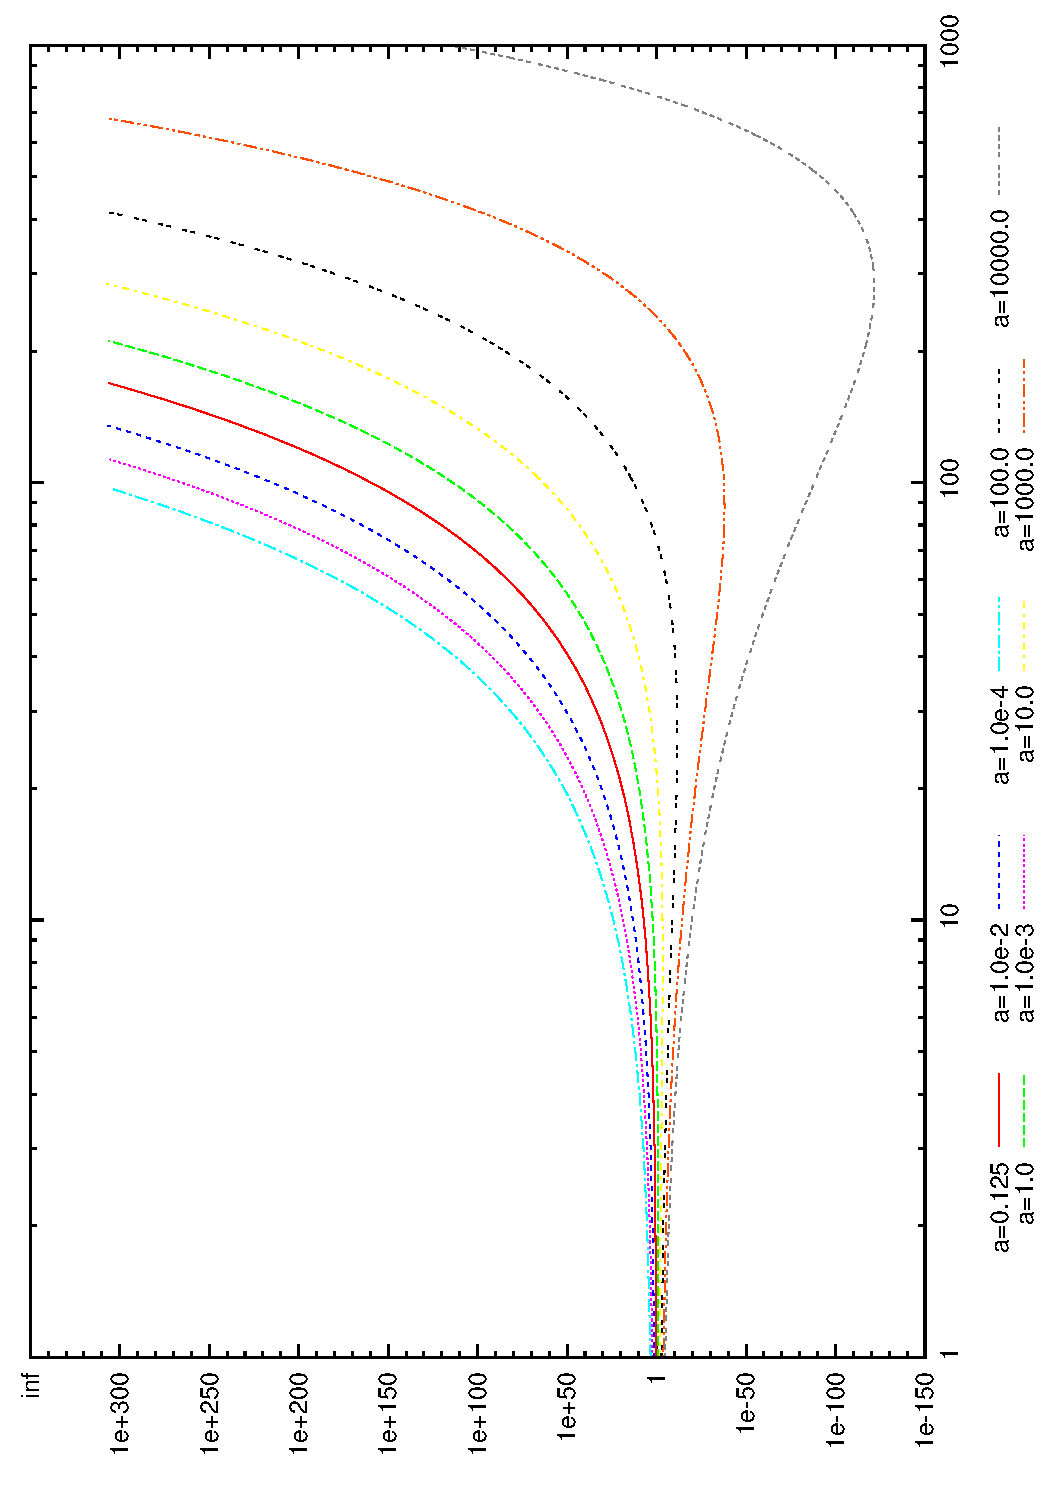
\includegraphics[angle=270,width=\the\textwidth]{../img/koeff.pdf}
  %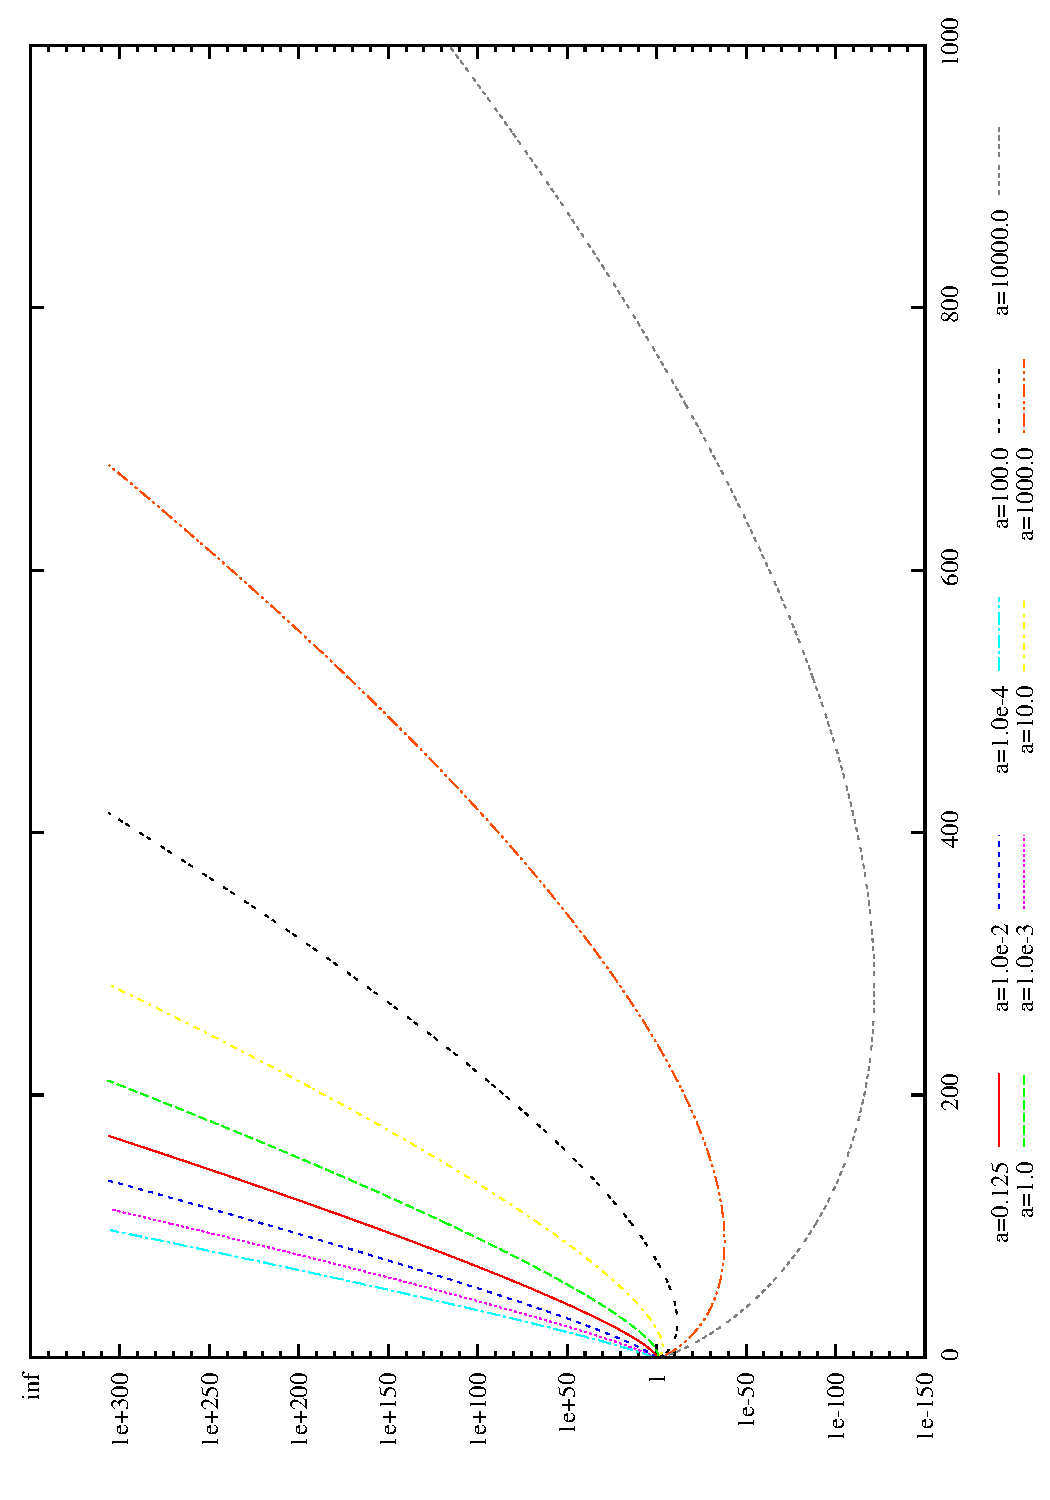
\includegraphics[angle=270,width=\the\textwidth]{../img/koeff-logx.pdf}
  \caption[Koeffizienten in abhängigkeit von $a$]
   {Die Beträge der Koeffizienten für unterschiedliche $a$}
  \label{fig:plotKoeffs}
\end{figure}

% vim: set ft=tex :
